\chapter{Results}
\label{capitulo5}

In this chapter the results collected from the Chapter 4 will be discussed and analyzed. It is important to freeze that only the approach 3 from \ref{sub:3} was implemented into the framework, due to the goal was to work with multiple cameras and multi-view perspective.

The algorithms and the simulations was performed in a computer with this follow configuration:

\begin{itemize}
    \item Operational System Ubuntu 18.04
    \item CPU Intel core i7 7700HQ 2.80 GHz
    \item 32 GB memory RAM
    \item GPU Nvidia Geforce GTX 1050 Ti - 4 GB
\end{itemize}


The idea of the framework is to perform the tests on Audi test track as shown in Figure \ref{fig:test_track}, but in this work only the proof of concept of the algorithms was performed. 

\begin{figure}[H]
\centering
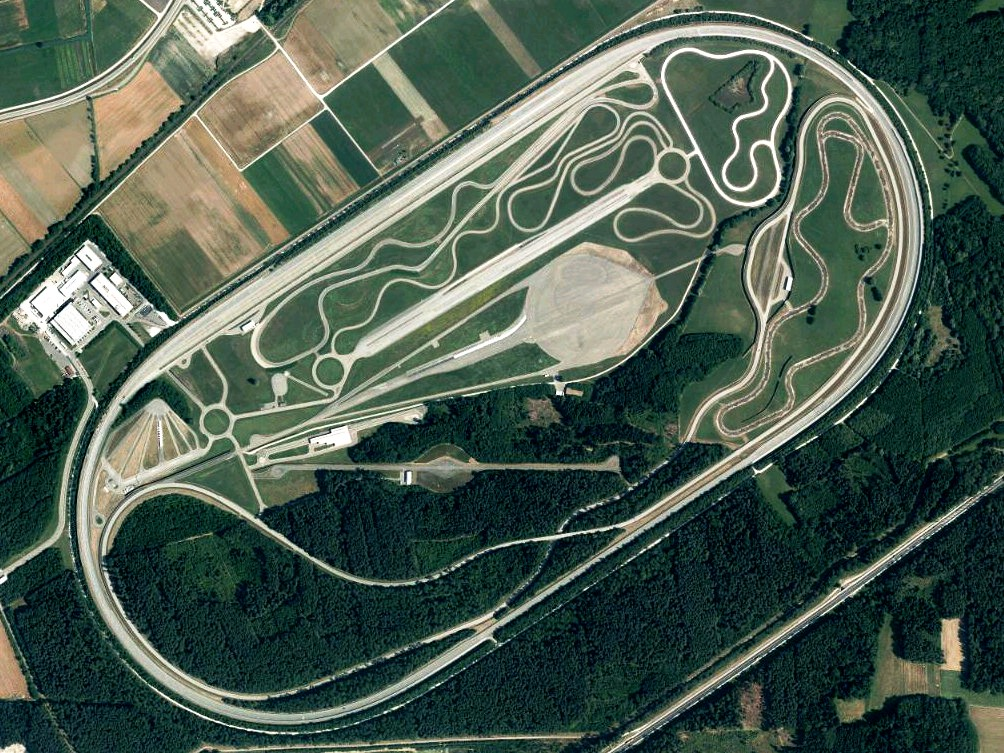
\includegraphics[scale=0.3]{imagens/testtrack.jpg}
\caption{Audi test track in eagle's view}
\label{fig:test_track}
\end{figure}


The algorithm for object detection was performed over the parking lot of the company EFS GmbH as shown in Figure \ref{fig:park}.


\begin{figure}[H]
\centering
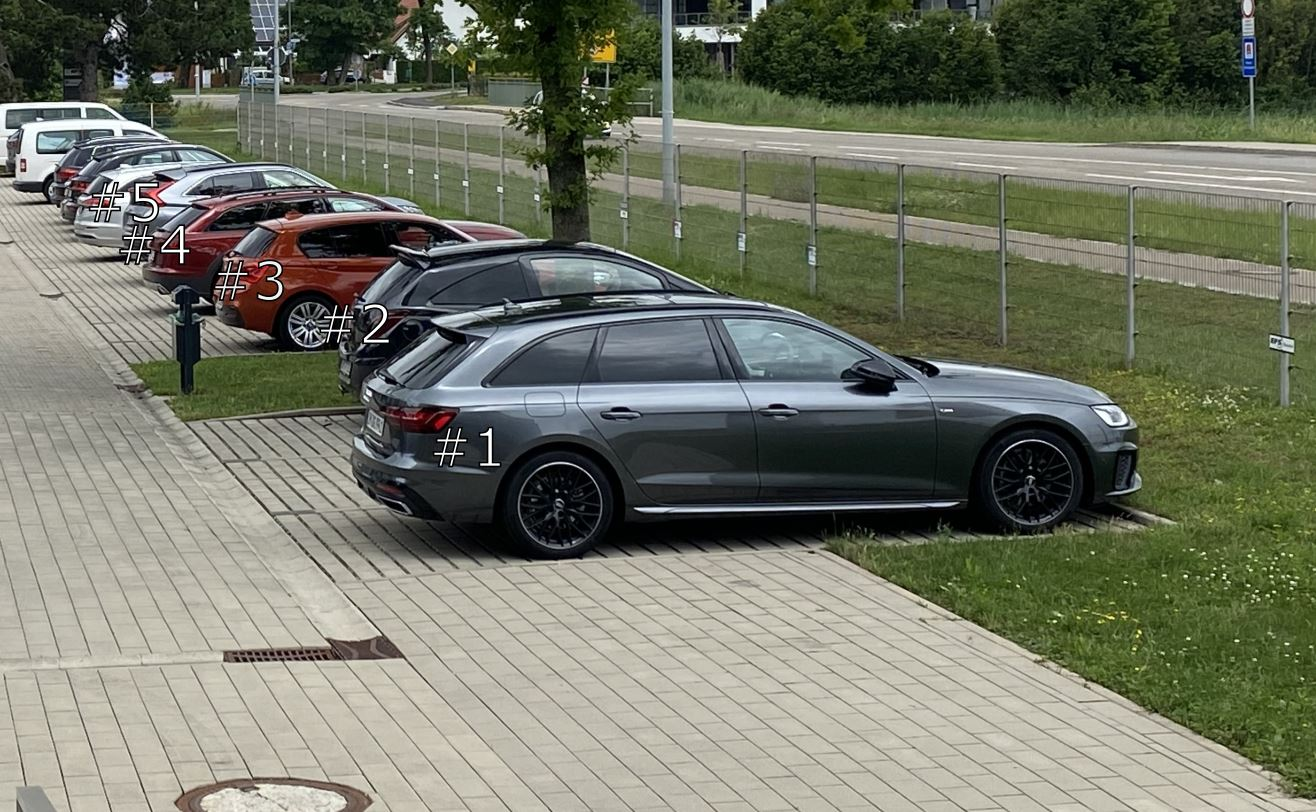
\includegraphics[scale=0.5]{imagens/park.JPG}
\caption{Position of the cars on the parking lot}
\label{fig:park}
\end{figure}

\section{Description of the test scenario}

The test scenario was built three times using different perspectives, for the first test where was necessary just to use the camera calibration perspective was built using only one camera and the height of this camera does not matter to compute the distance, only a known distance and dimensions of a known object to adjust this algorithm.

For the second scenario some photos was taken and labeled with the known metrics to support the training step and return a good result according with reality. 

The last approach and used in this work to built the framework was used following some principles as the cameras should be mounted at the same level, the same horizontal position,  the stream must be captured at the same time of the camera and sent to the same control center to process this data. 

The used cameras were GoPro 5 which allow to built a wireless network with many cameras 


\section{Results with camera calibration}

The results provided from the approach 1 from \ref{sub:1} was implemented using Python 3.7 and Opencv3, and the position was computed based the camera calibration. In (\ref{eq:focal_distance}) is defined the distance used to calibrate the camera, this step has been done with a measurer tape and a piece of paper ($21.59$ cm x  $27.94$ cm) and this was positioned $60.96$ cm in front of the camera to take the photo.

\begin{equation}
    \label{eq:focal_distance}
    F = \frac{P\cdot D}{W}
\end{equation}

where W is the width of the piece of the paper, in this case is $27.94$ cm, D is distance from the piece of paper to the camera, and P is the measure of the paper in pixels, this is taken from image. Applying the (\ref{eq:focal_distance}), the focal length (F) is $541.09$ pixels.





The results achieved with this technique is shown in Table \ref{tab:output_calibrate}. 

\begin{table}[H]
\centering
\caption{Measurements achieved with camera calibration algorithm}
\begin{tabular}{l|l} 
\toprule
Car &  Measurements      \\
\#1   & 4.05        \\
\#2   & 10.67       \\
\#3   & 15.52       \\
\#4   & 19.55       \\
\#5   & 20.08       \\
\bottomrule
\end{tabular}
\label{tab:output_calibrate}
\end{table} 



\section{Results with known map}
In this section is detailed the results of the proposal with known map, this approach was performed using the neural network from \ref{sub:2} and the data provided from KITTI Dataset \cite{geiger2013vision}, it is important to freeze, this approach was used only for comparison method and not to be used on the final framework. 


The results collected in this section are very useful, as several companies and other universities are releasing the dataset as open source. With this, there is a need to understand how to manipulate a set of images, and in some cases even data from RADAR and LIDAR are available.

The main ideia of this test was to get the information from the object detection performed with the algorithm using boundary boxes approach and collect this known information as input in the neural network and start to predict a distance from the camera until the object. Where in Figure \ref{fig:output} is shown an example of the known KITTI dataset, it serves just as motiviation for this work, the final results were not performed over this dataset. 

\begin{figure}[H]
\centering
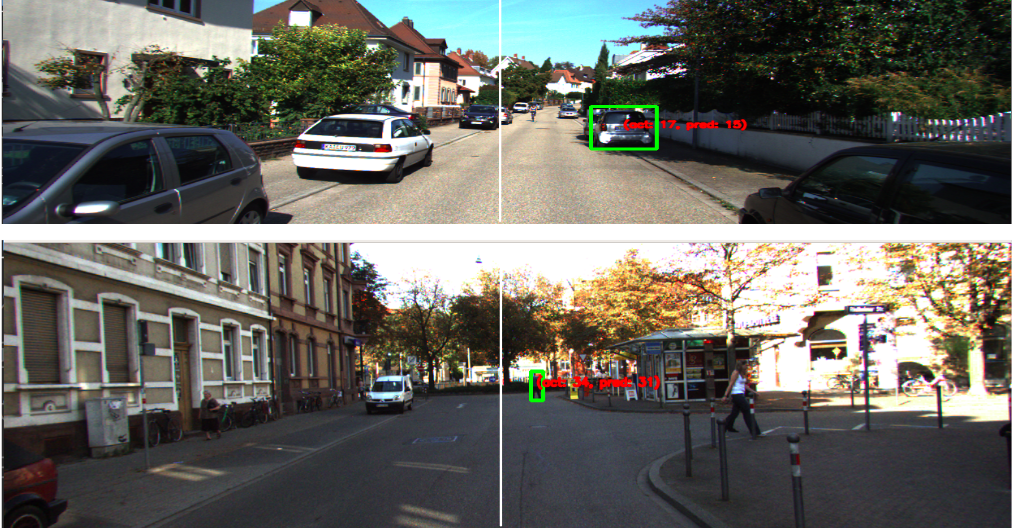
\includegraphics[width=\textwidth]{imagens/ouput.png}
\caption{Output results from framework using single stereo camera and known map}
\label{fig:output}
\end{figure}

For this approach the output achieved from Table \ref{tab:output_table} was used for the first interaction and estimate the distance as shown in Table \ref{tab:output_2}. These results are a little bit similar with the reality because the map is already known and the measurement step of these structures was performed and the labelling part as well.

\begin{table}[H]
\centering
\caption{Measurements achieved with camera and known map}
\begin{tabular}{l|l} 
\toprule
Car &  Measurements      \\
\#1   & 4.43        \\
\#2   & 10.98       \\
\#3   & 16.01       \\
\#4   & 18.99       \\
\#5   & 22.18       \\
\bottomrule
\end{tabular}
\label{tab:output_2}
\end{table} 


\section{Results with multicameras and proposed framework}


The algorithm of the proposed framework predict the objects of the whole scenario in 28 ms and has identified 9 cars on the image as show in Figure \ref{fig:park_predict} and in Table \ref{tab:accuracy} is shown the accuracy of each prediction for each car. The output accuracies from the algorithm are shown in Table \ref{fig:framework_predict}, the low accuracies are related with the partial occluded objects, such as the car 2 and car 6. 

The perspective of the distance, this algorithm computed this using the Inverse Perspective Mapping (IPM) combined with Yolo Algorithm, where the perspective of distance was fused on the last fully connecte layer. In Table \ref{tab:output_framework} is shown the results achieved from the perspective using two cameras. 

\begin{table}[H]
\centering
\caption{Measurements achieved with multicameras}
\begin{tabular}{l|l} 
\toprule
Car &  Measurements      \\
\#1   & 4.40        \\
\#2   & 11.05       \\
\#3   & 16.01       \\
\#4   & 19.92       \\
\#5   & 24.08       \\
\bottomrule
\end{tabular}
\label{tab:output_framework}
\end{table} 
 

In Figure \ref{fig:park_predict} was used just the model that contains the object recognition and detection using a single image and not as stream, this test was performed to see the accuracy of the algorithm in this purpose and identify how far is possible to detect the objects in this scenario, it is necessary to note that this test previewed only 5 cars to detection and the algorithm detect the whole cars in the scenario, each accuracy for each car of the test is available in Table \ref{tab:accuracy}.


\begin{figure}[H]
\centering
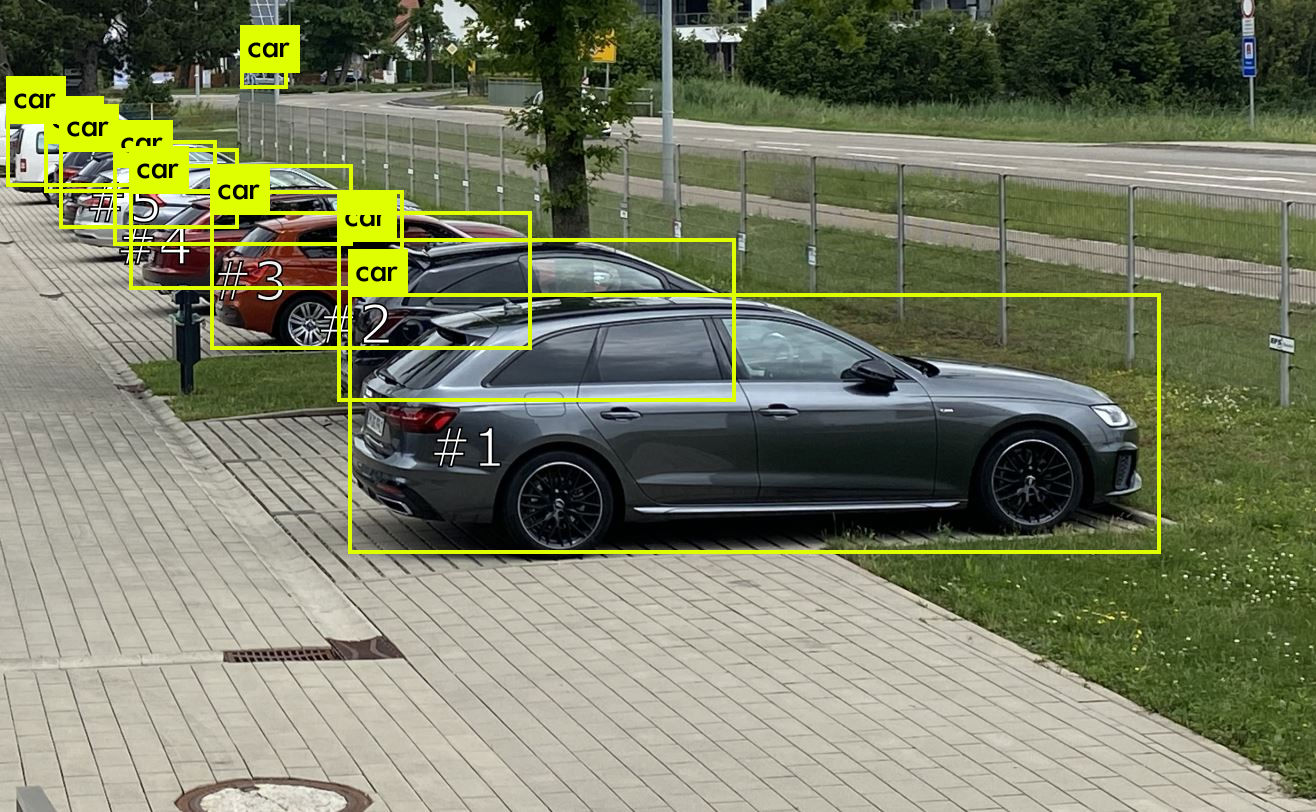
\includegraphics[scale=0.3]{imagens/predictions.jpg}
\caption{Output image with boundary boxes predictions}
\label{fig:park_predict}
\end{figure}



\begin{table}[H]
\centering
\caption{Accuracy of the proposed framework in object detector and classification}
\begin{tabular}{c|c}
\hline
Predicted Label & Accuracy \\ \hline
Car             & 91\%     \\ \hline
Car             & 31\%     \\ \hline
Car             & 96\%     \\ \hline
Car             & 94\%     \\ \hline
Car             & 95\%     \\ \hline
Car             & 98\%     \\ \hline
Car             & 47\%     \\ \hline
Car             & 97\%     \\ \hline
Car             & 98\%     \\ \hline
\end{tabular}
\label{tab:accuracy}
\end{table}



In Figure \ref{fig:framework_predict} is shown the frontend of the application of this work, it was developed using Python and Javascript to allow the browser communicate with the model. The Python module is composed by the libraries called sockets, and it permits the communication over many cameras and share the stream information between the cameras and the command central, it was possible because the cameras used in the tests have internal wireless network. And based on it a script with a proxy function was developed to take care of this behavior. 

The backend side of this project is described in the Appendix \ref{ap:app} where there are the information about the pre-processing step, training step, object detection, and the frontend scenario as well. The network was built using the framework Pytorch \cite{paszke2019pytorch} this script permits the abstraction of the Darknet to perform the object detection and the object recognition, and with all of this information the step to predict the distance was combined to show the output. 

The camera 1 of the Figure \ref{fig:framework_predict} is used only to perform the boundary boxes detection and the camera 2 is used to perform the distance prediction. This solution was embedded in a module to work as a controller of this framework.

% The experiments led us also to measure the rapidity of the multicameras method by computing the number of frames treated per second.  The Fig. 9 shows that the method could treat up to 23 frames per second. the average of frames per second through all the experiments is 20.57 frames per second which is enough for real time treatments. 

\begin{figure}[H]
\centering
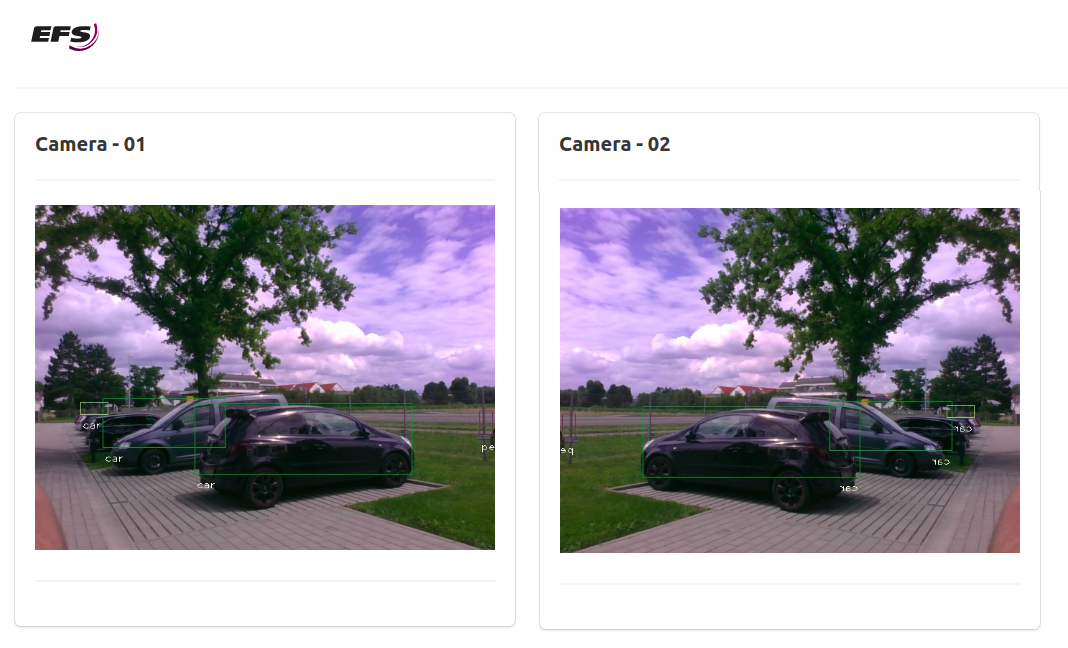
\includegraphics[scale=0.8]{imagens/output_framework.png}
\caption{Output image with predictions }
\label{fig:framework_predict}
\end{figure}



\section{Validation}

For validation purpose, it was used a commercial laser measurement as shown in Figure \ref{fig:laser_meas}, this model is known as Bosch DLE 40 Professional {\tiny{\textregistered}}. 



\begin{figure}[H]
\centering
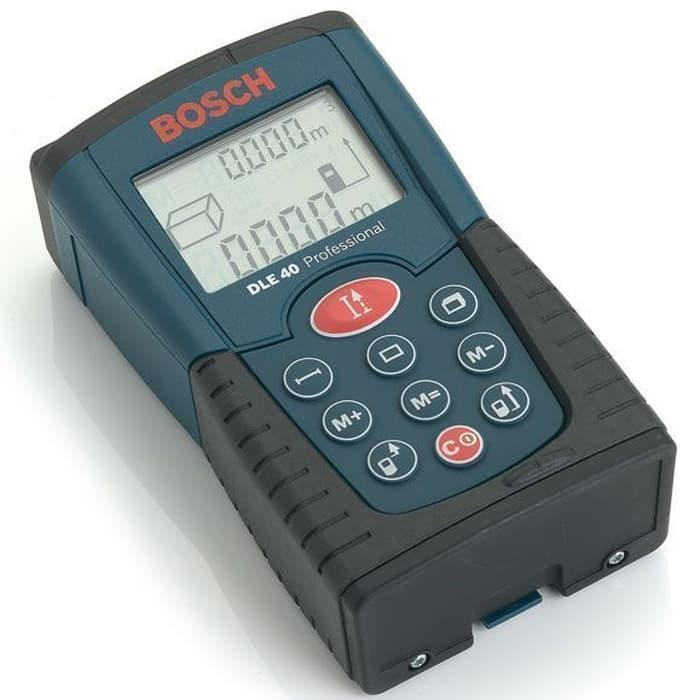
\includegraphics[scale=0.3]{imagens/trena.jpg}
\caption{Commercial laser measurer}
\label{fig:laser_meas}
\end{figure}

The instrumental error rate is $\pm 1.5 mm$, thereby we repeated the measure three times and computed the mean, and standard deviation as well. In Table \ref{tab:tab_measure} is shown the measurements with the camera positioned at $2.01$ m from the ground. And in Figure \ref{fig:park} is shown the position of the cars along the parking lot. The reason to measure three times is because in the manual is written that in sunny days can bias the measurement. 



\begin{table}[H]
\centering
\caption{Measurements collected with a commercial measurer}
\begin{tabular}{l|l|l|l|l} 
\toprule
Car & First measure (m) & Second measure (m) & Third measure (m) & Mean (m) \\
\#1   & 4.25          & 4.47           & 4.51           & 4.41 \\
\#2   & 11.01         & 11.21          & 11.11          & 11.11\\
\#3   & 16.12         & 16.35          & 16.26          & 16.24\\
\#4   & 19.63         & 19.69          & 19.66          & 19.66\\
\#5   & 23.08         & 23.18          & 23.01          & 23.09\\
\bottomrule
\end{tabular}
\label{tab:tab_measure}
\end{table} 


For purpose to comparison and to see the differences between the approaches and the real distance computed with the tool from Figure \ref{fig:laser_meas}. The Table \ref{tab:total} was built to facilitate the visualization of these outputs. 


\begin{table}[H]
\centering
\caption{Comparison between the algorithms and real data}
\begin{tabular}{l|l|l|l|l} 
\toprule
Car & Camera Calibration (m) & Known Map (m) & Multicameras (m) & Real distance (m) \\
\#1   & 4.05          & 4.43           & \textbf{4.40 }          & 4.41 \\
\#2   & 10.67         & 10.98          & \textbf{11.05 }         & 11.11\\
\#3   & 15.52         & \textbf{16.01}          &\textbf{ 16.01 }         & 16.24\\
\#4   & \textbf{19.55}         & 18.99          & 19.92          & 19.66\\
\#5   & 20.08         & 22.18          & \textbf{24.08}          & 23.09\\
\bottomrule
\end{tabular}
\label{tab:total}
\end{table} 

For to analyze the difference between the implemented methods, it is necessary to examine the error between the real value. For this a Python script was implement using Pandas Library \cite{mckinney2011pandas} to take care of the collected data. The error analysis was implemented to make it easier the visualization of the best applied technique. 

The pre-processed samples are used as input for the algorithms under text, resulting in estimations of the true position value. Results are expressed in terms of the RMSE, given by (\ref{eq:rmse}):
%
\begin{equation} \label{eq:rmse}
\text{RMSE}(f, \hat{f}) = \sqrt{\frac{1}{n_\text{samples}} \sum_{i=0}^{n_\text{samples} - 1} (f_i - \hat{f}_i)^2},
\end{equation}
%
calculated for each estimator $\hat{f}_i$, referenced either from the measurement tool of Figure \ref{fig:laser_meas} true value $f_i$ as read at the end of each measurement.

In Figure \ref{fig:rmse} is shown a chart with the three proposed techniques using (\ref{eq:rmse}), where is possible to see in certain points the multicameras approach was better and the camera calibration was the worse approach for this case. 

\begin{figure}[H]
\centering
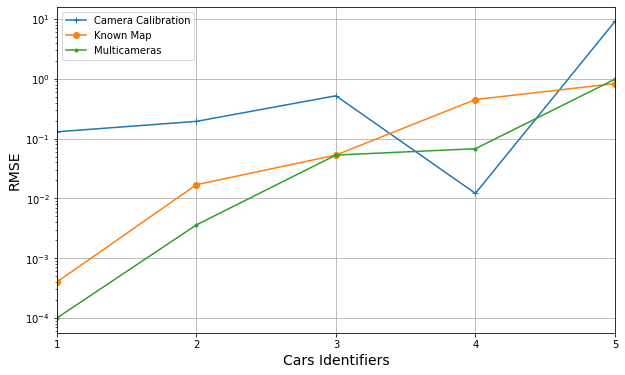
\includegraphics[scale=0.6]{imagens/plot.png}
\caption{RMSE of estimated estimate position for each algorithm for different detected car, referenced to values measured by the commercial laser measurer}
\label{fig:rmse}
\end{figure}